\documentclass[]{article}
\usepackage{lmodern}
\usepackage{amssymb,amsmath}
\usepackage{ifxetex,ifluatex}
\usepackage{fixltx2e} % provides \textsubscript
\ifnum 0\ifxetex 1\fi\ifluatex 1\fi=0 % if pdftex
  \usepackage[T1]{fontenc}
  \usepackage[utf8]{inputenc}
\else % if luatex or xelatex
  \ifxetex
    \usepackage{mathspec}
  \else
    \usepackage{fontspec}
  \fi
  \defaultfontfeatures{Ligatures=TeX,Scale=MatchLowercase}
\fi
% use upquote if available, for straight quotes in verbatim environments
\IfFileExists{upquote.sty}{\usepackage{upquote}}{}
% use microtype if available
\IfFileExists{microtype.sty}{%
\usepackage{microtype}
\UseMicrotypeSet[protrusion]{basicmath} % disable protrusion for tt fonts
}{}
\usepackage[margin=1in]{geometry}
\usepackage{hyperref}
\hypersetup{unicode=true,
            pdftitle={Module 6 - Publications reproductibles avec RMarkdown},
            pdfauthor={Groupe des référents R},
            pdfborder={0 0 0},
            breaklinks=true}
\urlstyle{same}  % don't use monospace font for urls
\usepackage{color}
\usepackage{fancyvrb}
\newcommand{\VerbBar}{|}
\newcommand{\VERB}{\Verb[commandchars=\\\{\}]}
\DefineVerbatimEnvironment{Highlighting}{Verbatim}{commandchars=\\\{\}}
% Add ',fontsize=\small' for more characters per line
\usepackage{framed}
\definecolor{shadecolor}{RGB}{248,248,248}
\newenvironment{Shaded}{\begin{snugshade}}{\end{snugshade}}
\newcommand{\KeywordTok}[1]{\textcolor[rgb]{0.13,0.29,0.53}{\textbf{#1}}}
\newcommand{\DataTypeTok}[1]{\textcolor[rgb]{0.13,0.29,0.53}{#1}}
\newcommand{\DecValTok}[1]{\textcolor[rgb]{0.00,0.00,0.81}{#1}}
\newcommand{\BaseNTok}[1]{\textcolor[rgb]{0.00,0.00,0.81}{#1}}
\newcommand{\FloatTok}[1]{\textcolor[rgb]{0.00,0.00,0.81}{#1}}
\newcommand{\ConstantTok}[1]{\textcolor[rgb]{0.00,0.00,0.00}{#1}}
\newcommand{\CharTok}[1]{\textcolor[rgb]{0.31,0.60,0.02}{#1}}
\newcommand{\SpecialCharTok}[1]{\textcolor[rgb]{0.00,0.00,0.00}{#1}}
\newcommand{\StringTok}[1]{\textcolor[rgb]{0.31,0.60,0.02}{#1}}
\newcommand{\VerbatimStringTok}[1]{\textcolor[rgb]{0.31,0.60,0.02}{#1}}
\newcommand{\SpecialStringTok}[1]{\textcolor[rgb]{0.31,0.60,0.02}{#1}}
\newcommand{\ImportTok}[1]{#1}
\newcommand{\CommentTok}[1]{\textcolor[rgb]{0.56,0.35,0.01}{\textit{#1}}}
\newcommand{\DocumentationTok}[1]{\textcolor[rgb]{0.56,0.35,0.01}{\textbf{\textit{#1}}}}
\newcommand{\AnnotationTok}[1]{\textcolor[rgb]{0.56,0.35,0.01}{\textbf{\textit{#1}}}}
\newcommand{\CommentVarTok}[1]{\textcolor[rgb]{0.56,0.35,0.01}{\textbf{\textit{#1}}}}
\newcommand{\OtherTok}[1]{\textcolor[rgb]{0.56,0.35,0.01}{#1}}
\newcommand{\FunctionTok}[1]{\textcolor[rgb]{0.00,0.00,0.00}{#1}}
\newcommand{\VariableTok}[1]{\textcolor[rgb]{0.00,0.00,0.00}{#1}}
\newcommand{\ControlFlowTok}[1]{\textcolor[rgb]{0.13,0.29,0.53}{\textbf{#1}}}
\newcommand{\OperatorTok}[1]{\textcolor[rgb]{0.81,0.36,0.00}{\textbf{#1}}}
\newcommand{\BuiltInTok}[1]{#1}
\newcommand{\ExtensionTok}[1]{#1}
\newcommand{\PreprocessorTok}[1]{\textcolor[rgb]{0.56,0.35,0.01}{\textit{#1}}}
\newcommand{\AttributeTok}[1]{\textcolor[rgb]{0.77,0.63,0.00}{#1}}
\newcommand{\RegionMarkerTok}[1]{#1}
\newcommand{\InformationTok}[1]{\textcolor[rgb]{0.56,0.35,0.01}{\textbf{\textit{#1}}}}
\newcommand{\WarningTok}[1]{\textcolor[rgb]{0.56,0.35,0.01}{\textbf{\textit{#1}}}}
\newcommand{\AlertTok}[1]{\textcolor[rgb]{0.94,0.16,0.16}{#1}}
\newcommand{\ErrorTok}[1]{\textcolor[rgb]{0.64,0.00,0.00}{\textbf{#1}}}
\newcommand{\NormalTok}[1]{#1}
\usepackage{graphicx,grffile}
\makeatletter
\def\maxwidth{\ifdim\Gin@nat@width>\linewidth\linewidth\else\Gin@nat@width\fi}
\def\maxheight{\ifdim\Gin@nat@height>\textheight\textheight\else\Gin@nat@height\fi}
\makeatother
% Scale images if necessary, so that they will not overflow the page
% margins by default, and it is still possible to overwrite the defaults
% using explicit options in \includegraphics[width, height, ...]{}
\setkeys{Gin}{width=\maxwidth,height=\maxheight,keepaspectratio}
\IfFileExists{parskip.sty}{%
\usepackage{parskip}
}{% else
\setlength{\parindent}{0pt}
\setlength{\parskip}{6pt plus 2pt minus 1pt}
}
\setlength{\emergencystretch}{3em}  % prevent overfull lines
\providecommand{\tightlist}{%
  \setlength{\itemsep}{0pt}\setlength{\parskip}{0pt}}
\setcounter{secnumdepth}{0}
% Redefines (sub)paragraphs to behave more like sections
\ifx\paragraph\undefined\else
\let\oldparagraph\paragraph
\renewcommand{\paragraph}[1]{\oldparagraph{#1}\mbox{}}
\fi
\ifx\subparagraph\undefined\else
\let\oldsubparagraph\subparagraph
\renewcommand{\subparagraph}[1]{\oldsubparagraph{#1}\mbox{}}
\fi

%%% Use protect on footnotes to avoid problems with footnotes in titles
\let\rmarkdownfootnote\footnote%
\def\footnote{\protect\rmarkdownfootnote}

%%% Change title format to be more compact
\usepackage{titling}

% Create subtitle command for use in maketitle
\newcommand{\subtitle}[1]{
  \posttitle{
    \begin{center}\large#1\end{center}
    }
}

\setlength{\droptitle}{-2em}

  \title{Module 6 - Publications reproductibles avec RMarkdown}
    \pretitle{\vspace{\droptitle}\centering\huge}
  \posttitle{\par}
    \author{Groupe des référents R}
    \preauthor{\centering\large\emph}
  \postauthor{\par}
      \predate{\centering\large\emph}
  \postdate{\par}
    \date{19 janvier 2019}


\begin{document}
\maketitle

\section{Introduction}\label{introduction}

\subsection{Le parcours de formation}\label{le-parcours-de-formation}

Le parcours de formation proposé est structuré en modules de 2 jours
chacun :

\begin{itemize}
\tightlist
\item
  1 : Socle de base \(\Rightarrow\)
  \href{https://rawgit.com/MTES-MCT/parcours-r/master/Supports_formations/m1_socle/_book/index.html}{support}
\item
  2 : Préparer ses données avec le tidyverse \(\Rightarrow\)
  \href{https://rawgit.com/MTES-MCT/parcours-r/master/Supports_formations/m2_preparation_donnees/_book/index.html}{support}
\item
  3 : Statistiques descriptives \(\Rightarrow\)
  \href{https://rawgit.com/MTES-MCT/parcours-r/master/Supports_formations/m3_stats_desc/_book/index.html}{support}
\item
  4 : Analyses multivariées \(\Rightarrow\)
  \href{https://rawgit.com/MTES-MCT/parcours-r/master/Supports_formations/m4_analyse_donnees/_book/index.html}{support}
\item
  5 : Datavisualisation : Produire des graphiques, des cartes et des
  tableaux \(\Rightarrow\)
  \href{https://rawgit.com/MTES-MCT/parcours-r/master/Supports_formations/m5_valorisation_des_donnees/_book/index.html}{support}
\item
  6 : Documents reproductibles avec RMarkdown (2\textsuperscript{ème}
  semestre 2019)
\end{itemize}

\ldots{} et en perspective : analyse spatiale, applis interactives avec
Shiny, big data, etc.

Pour vous tenir au courant de l'offre de formation proposée par le
réseau des CVRH, \href{http://oups-cmvrh.e2.rie.gouv.fr/}{consultez la
plateforme OUPS}. Vous pouvez vous y abonner pour recevoir les annonces
qui vous intéressent.

Il existe une liste pour diffuser de l'information, échanger autour de R
ou lever des points de blocage. Pour s'insrire, envoyer un message vide
avec le titre ``subscribe labo.communaute-r'' à l'adresse
\href{mailto:sympa@developpement-durable.gouv.fr}{\nolinkurl{sympa@developpement-durable.gouv.fr}}.

\subsection{La publication
reproductible}\label{la-publication-reproductible}

Ajouter des sources ? (\url{https://rmarkdown.rstudio.com/}) La
cheatsheet :
\url{https://www.rstudio.com/wp-content/uploads/2016/03/rmarkdown-cheatsheet-2.0.pdf}

Le schéma classique pour produire un rapport ou une publication
ressemble à ça :

\begin{figure}
\centering
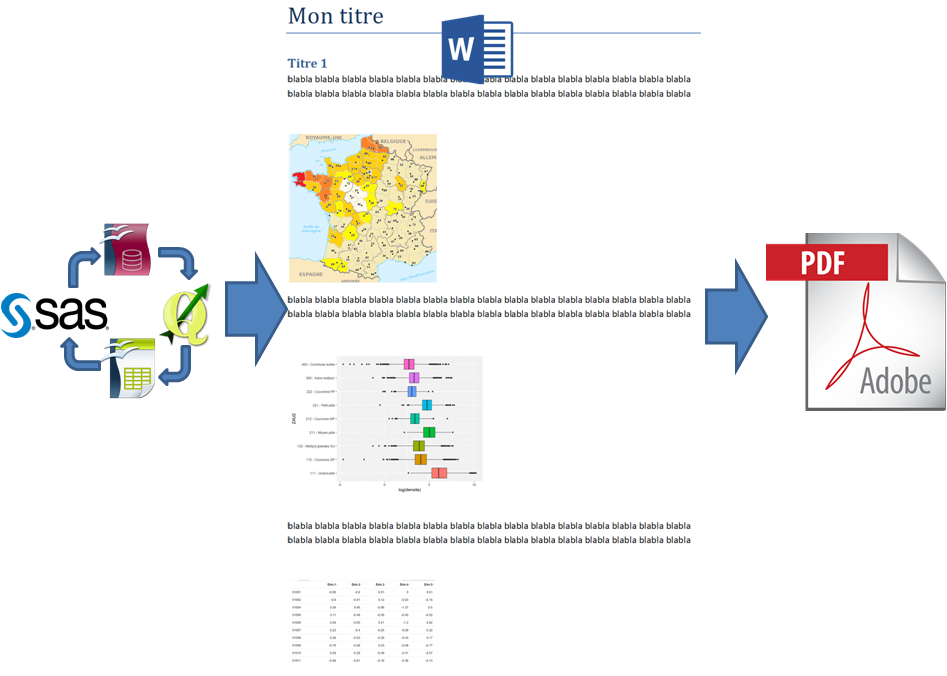
\includegraphics{images/schema_publi.png}
\caption{}
\end{figure}

Les données mobilisées proviennent de bases de données, de tables ou de
SIG, et rien que pour les lire, il y a besoin de plusieurs logiciels
selon les formats.

Les données sont ensuite nettoyées (valeurs manquantes ou aberrantes,
recodages, discrétisation, renommages \ldots{}), puis traitées
(sélection, agrégation, modélisation) et visualisées (tables,
graphiques, cartes). Les éléments visuels sont insérés dans un
traitement de texte qui sert aussi à la rédaction, et enfin la version
diffusable est produite au format pdf.

Plusieurs inconvénients à cette chaîne d'opérations :

\begin{itemize}
\tightlist
\item
  Beaucoup d'opérations manuelles chronophages et sources potentielles
  d'erreurs.
\item
  Si quelque chose change, il faut tout recommencer (mise à jour,
  adaptation à une autre zone géographique ou fenêtre temporelle).
\item
  La publication finale n'est pas ``reproductible'' au sens où la
  traçabilité est insuffisante pour qu'un autre auteur, avec les mêmes
  données, arrive à la même publication \(\Rightarrow\) la recherche
  d'erreurs est difficile et les passations délicates.
\item
  Les contenus sont statiques, ce qui est peu attractif par rapport aux
  possibilités d'interactivité offertes par les technologies web.
\end{itemize}

Le fil conducteur de ce module est la production de A à Z d'un portrait
de territoire, à partir de données variées, en travaillant entièrement
dans RStudio au format R Markdown.

\subsection{\texorpdfstring{Le format ``R
Markdown''}{Le format R Markdown}}\label{le-format-r-markdown}

Ce format de document a été introduit en 2012 à la sortie du package
\texttt{knitr}.

Auparavant, il existait Markdown, un ``langage de balisage léger'',
sorte d'intermédiaire entre du texte brut et du traitement de texte. La
syntaxe de Markdown est très simplifiée. On peut le saisir avec un
éditeur de texte comme \emph{Notepad} et il est lisible même non
formaté.

Pourquoi utiliser un langage de balisage léger ? Des avantages majeurs :

\begin{itemize}
\tightlist
\item
  Séparer le fond de la forme. On peut taper ``au kilomètre'' en se
  concentrant sur le contenu, et voir ensuite les questions de forme (y
  compris le format de sortie, HTML, PDF, traitements de texte,
  diaporamas, tableaux de bord, voire EPUB).
\item
  Cette simplicité permet le suivi de version par des outils comme
  \href{https://fr.wikipedia.org/wiki/Git}{Git}.
\end{itemize}

Par contre, la simplicité signifie peu de fonctionnalités donc des
sorties assez pauvres.

L'idée, avec R Markdown, était garder les avantages du langage existant
Markdown mais en lui ajoutant des fonctionnalités d'interprétation de
code R, intégré aux documents sous formes de \texttt{chunks}. En fait,
les versions actuelles du package \texttt{knitr} permettent
d'interpréter d'autres langages comme du \(\LaTeX\) ou du code Python.

R Markdown est en quelque sorte un cadre pour travailler en data
science. Un même document permet de sauvegarder et exécuter du code
ainsi que de produire des rapports mis en forme pouvant contenir une
grande diversité d'objets statiques ou dynamiques.

\section{Le fichier R Markdown}\label{le-fichier-r-markdown}

\subsection{Nouveau fichier}\label{nouveau-fichier}

Extension du fichier

\subsection{Structure}\label{structure}

Un fichier R Markdown est constitué de 3 éléments principaux.

\begin{figure}
\centering
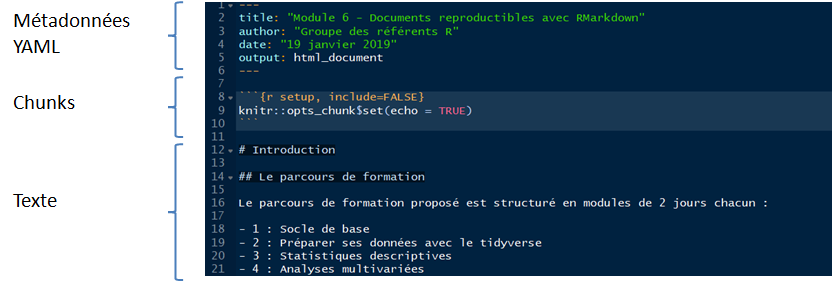
\includegraphics{images/script.png}
\caption{}
\end{figure}

Les métadonées permettent une meilleure tracabilité des codes, de suivre
les mises à jour ainsi que de choisir le type de format de sortie que
l'on souhaite avoir (PDF, HTML, DOCX). Les chunks sont des composants
permettant l'execution de codes R, mais aussi de plusieurs autres
langages de programmation (Python, SQL \ldots{}). La partie texte peut
contenir, en plus du texte, divers éléments qui peuvent être interprétés
comme des balises HTML ou du code \(\LaTeX\) ou CSS.

\subsection{Du .Rmd au format de
sortie}\label{du-.rmd-au-format-de-sortie}

\begin{figure}
\centering
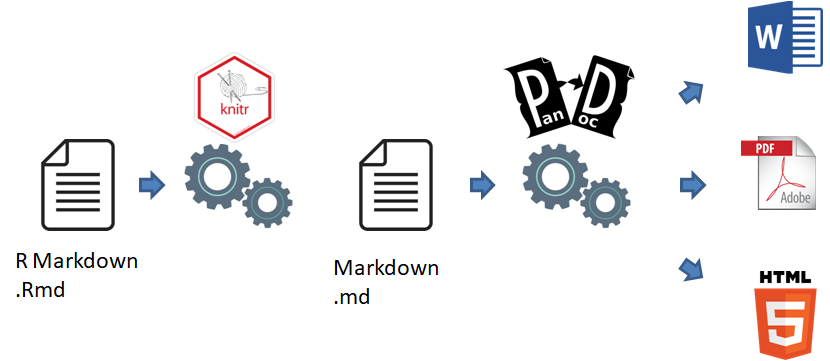
\includegraphics{images/render.png}
\caption{}
\end{figure}

On distingue deux étapes :

\begin{itemize}
\tightlist
\item
  La première, réalisée par le package knitr, interprète le document R
  Markdown et exécute les chunks. Elle produit un fichier Markdown
  contenant le texte, le code et le résultat de l'exécution du code.
\item
  Puis, le convertisseur de formats Pandoc se charge de produire le
  document de sortie au format choisi.
\end{itemize}

Ca peut paraître compliqué mais en pratique, chacune des fonctions
\texttt{render} de \texttt{knitr} exécute la chaîne du début à la fin.

\section{Les différents éléments d'un fichier
.Rmd}\label{les-differents-elements-dun-fichier-.rmd}

\subsection{Les titres}\label{les-titres}

\subsection{Insérer des images}\label{inserer-des-images}

dimensions Lien. Stockage dans un sous-répertoire.

\subsection{Insérer des liens
hypertexte}\label{inserer-des-liens-hypertexte}

\subsection{Insérer du code}\label{inserer-du-code}

Il est possible d'insérer directement les résultats d'un code dans le
texte d'un fichier .Rmd en entourant le code d'un \texttt{r}.

\subsection{Insérer des éléments en
LaTeX}\label{inserer-des-elements-en-latex}

\(\LaTeX\) permet de mettre en forme toutes les expressions
mathématiques.

\subsection{}\label{section}

\section{Paramétrage général du fichier
.Rmd}\label{parametrage-general-du-fichier-.rmd}

Dimension, format de sortie, table des matière, css, yml,

\section{Les chunks}\label{les-chunks}

Raccourcis d'insersion d'un chunk : Ctrl + Alt + I

\subsection{Les options des chunks}\label{les-options-des-chunks}

include = FALSE : permet de ne pas afficher le code et ses résultats
lorsque le fichier est complété. Le code contenu dans le chunk est
cependant bien éxecuté par R Markdown et les résultats sont utilisables
par d'autres chunks. echo = FALSE : permet de ne pas afficher les codes
dans le fichier final. Le résultat est par contre affiché. Cette option
est utile lorsqu'on veut intégrer des graphiques dans son fichier.
message = FALSE : empêche l'affichage des messages d'information générés
par les codes. warning = FALSE : empêche l'affichage des messages
d'alerte générés par les codes. fig.cap = ``\ldots{}'' : ajoute une
légende aux graphiques.

\subsection{Les options globales des
chunks}\label{les-options-globales-des-chunks}

Il est possible d'appliquer des options globales qui affecterons chacun
des chunks qui sont contenus dans le fichier. Il est bien évidemment
possible de modifier les options globales dans les options locales de
chacun des chunks.

\subsection{Le cache}\label{le-cache}

Si le temps d'éxecution du code est trop long, il est possible
d'utiliser l'option de mise en cache de knirt afin d'améliorer les
performances d'éxécution de votre code.

Enchaînement, paramétrage,

\section{}\label{section-1}

\section{A ne pas oublier}\label{a-ne-pas-oublier}

Utilisation backticks Latex Bookdown Balises Table des matières css
liens images versioning mise en page Flexdashboard nommer les chunks Les
thèmes ggplot pour assurer la présentation homogène des graphiques + les
fonctions custom

\section{Rappels du jour 1}\label{rappels-du-jour-1}

\section{Exercice}\label{exercice}

\subsection{Cadrage}\label{cadrage}

\subsubsection{Problématique}\label{problematique}

\subsubsection{Rendu}\label{rendu}

Pour ce rendu, quelles données ? Quels packages ? \#\#\# Données dispo

\subsection{Mise en page}\label{mise-en-page}

\subsubsection{Quel type ? Barre de navigation ou onglets
?}\label{quel-type-barre-de-navigation-ou-onglets}

\subsubsection{Un petit CSS}\label{un-petit-css}

\subsubsection{Logo}\label{logo}

\subsubsection{Métadoonnées}\label{metadoonnees}

\subsubsection{Dashboard}\label{dashboard}

\subsection{Importation des données}\label{importation-des-donnees}

\begin{Shaded}
\begin{Highlighting}[]
\NormalTok{data =}\StringTok{ }\KeywordTok{load}\NormalTok{(}\StringTok{"à remplir une fois qu'on aura choisi des données"}\NormalTok{) }
\end{Highlighting}
\end{Shaded}

\subsubsection{jointure des tables}\label{jointure-des-tables}

\subsubsection{Données tabulées}\label{donnees-tabulees}

\subsubsection{Requêter une API}\label{requeter-une-api}

\subsubsection{Données géo}\label{donnees-geo}

\subsection{Création des objets}\label{creation-des-objets}

\subsubsection{Tables}\label{tables}

packages DT,
\href{https://www.littlemissdata.com/blog/prettytables}{formattable}
Fonction knitr::kable et kableextra cf.~exemple {[}ici{]}
(\url{https://haozhu233.github.io/kableExtra/awesome_table_in_html.html})

\subsubsection{Graphiques}\label{graphiques}

Types de graphiques; interactivité plotly et highcharter

\subsubsection{Cartes}\label{cartes}

leaflet ; fond de carte OSM géolocalisation : corresp adresses-données
formats de cartes geojson, shp donnée ponctuelle, polygones

\subsection{Assemblage}\label{assemblage}

dimensions formats de sortie. Besoin de Latex ?

règles de semiologie dans m5 hébergement html tenir Thierry au courant


\end{document}
